\documentclass[sigconf, nonacm, onecolumn]{acmart}

\usepackage[utf8]{inputenc}
\usepackage[T1]{fontenc}
\usepackage{lmodern}  % scalable fonts required for pdfTeX font expansion under acmart
\usepackage{graphicx}
\usepackage{booktabs}
\usepackage{amsfonts}
\usepackage{nicefrac}
% \usepackage{microtype}  % disabled: triggers pdfTeX font-expansion error w/ MiKTeX default cm fonts
\usepackage{amsmath}

%% ----------------------------------------------------------------
%% Title
%% ----------------------------------------------------------------
\title{Mitigating Reasoning Hallucinations in LLMs via
Neuro-Symbolic Integration for Ill-Defined
Mathematical Problems}

%% ----------------------------------------------------------------
%% Authors
%% ----------------------------------------------------------------
\author{Jave Bacsain}
\affiliation{%
  \department{College of Computer Studies}
  \institution{Camarines Sur Polytechnic Colleges}
  \country{Philippines}
}
\email{javbacsain@my.cspc.edu.ph}

\author{Ivy Pauline Muit}
\affiliation{%
  \department{College of Computer Studies}
  \institution{Camarines Sur Polytechnic Colleges}
  \country{Philippines}
}
\email{ivmuit@my.cspc.edu.ph}

%% ----------------------------------------------------------------
\begin{document}

\begin{teaserfigure}
  \centering
  
\includegraphics[width=3cm]{logo.png}\\[4pt]
  {\small CSAC 224 -- Natural Language Processing}
\end{teaserfigure}

\maketitle

%% ----------------------------------------------------------------
\section{Abstract}

Large Language Models (LLMs) are powerful text-generation systems, but they
tend to produce confident yet incorrect answers when given mathematical problems
that are missing key information or contain contradictory conditions. This paper
proposes a hybrid system that combines a fine-tuned language model with an
external logic solver to address this limitation. The language model will be trained
to translate a math word problem written in plain English into a formal logical
description of its constraints. That description will then be handed to Z3, a
widely-used constraint-satisfaction tool, which will determine whether the problem
has a valid solution. If the constraints are contradictory or leave the problem
unsolvable, the system will output a ``Reject'' classification instead of guessing.
This design separates the task of \textit{understanding language} from the task of
\textit{solving logic}, which prevents the model from fabricating answers at the
reasoning stage.

%% ----------------------------------------------------------------
\section{Introduction}

Modern Large Language Models (LLMs), systems trained to predict the next word in a
sequence, have become surprisingly capable at answering questions in plain
language~\cite{brown2020}. However, they have a structural weakness: because they are
trained to produce \textit{plausible} text, they will often generate a confident-sounding
answer even when no correct answer exists~\cite{huang2025}. This tendency is known as
hallucination.

The problem is especially damaging in mathematics. Real-world applications in fields such
as finance, healthcare, and engineering frequently involve problems with missing data or
conflicting requirements~\cite{puchalska1987}. A student who forgets to include a key
value in their homework, or a dataset with an entry error, can produce a problem that is
mathematically unsolvable, yet standard LLMs will still produce a numeric answer with
apparent confidence.

This proposal aims to build a system that will recognize when a math problem is
ill-defined and refuse to guess, rather than hallucinate a wrong answer. The system will
take a math word problem written in plain English as input, and will output either a
numeric answer (if the problem is solvable) or a ``Reject'' label (if it is not). To do
this, the system will use a language model not to solve the problem directly, but to
describe the problem's logical structure in a format that an external solver can evaluate
rigorously.

This project is being submitted exclusively for this Natural Language Processing class and
its components have not been used for any other courses.

%% ----------------------------------------------------------------
\section{Related Work}

Prior work on improving the reasoning ability of language models can be grouped into three
categories: prompting strategies, tool-assisted approaches, and logic-based systems.

\textbf{Prompting Strategies.} Chain-of-Thought (CoT) prompting~\cite{wei2022} improved
language model reasoning by asking the model to write out intermediate steps before giving
a final answer, rather than jumping straight to a conclusion. This simple change
significantly improved accuracy on multi-step problems. Kojima et al.~\cite{kojima2022}
extended this idea by showing that a single fixed phrase, ``Let's think step by step,''
added before the model's answer could trigger the same step-by-step behavior without
needing hand-crafted examples for each task. Building on this, Program of Thoughts
(PoT)~\cite{chen2023} went further by having the model write a small Python program
instead of natural language steps, letting a code interpreter handle the arithmetic. This
removes a major source of calculation errors. MathPrompter~\cite{imani2023} pushed this
further still by generating multiple independent solutions to the same problem and
checking whether they agree before committing to an answer, which raises confidence in the
output. Lightman et al.~\cite{lightman2024} showed that providing feedback on each
individual reasoning step during training, rather than only on the final answer,
significantly reduces logical errors in multi-step problems. However, none of these
approaches addresses the case where a problem has no valid solution, and the model will
still attempt to produce an answer.

\textbf{Tool-Assisted Language Models.} A second line of work connects language models to
external tools. Program-Aided Language Models (PAL)~\cite{gao2023} delegate arithmetic
steps to a Python interpreter, reducing calculation mistakes. The Chameleon
framework~\cite{lu2023} treats the language model as a planner that decides which external
tool to call, including web search or rule-based modules, for each part of a problem.
ReAct~\cite{yao2023} takes a similar direction by interleaving reasoning steps with
real-world actions, such as looking up facts. Toolformer~\cite{schick2023} demonstrated
that a language model can be trained to decide on its own when to call an external tool
by inserting API calls directly into its training data. While these systems extend what a
language model can do, they are still oriented toward finding an answer, not toward
recognizing when an answer cannot exist.

\textbf{Formal Logic and Neuro-Symbolic Systems.} The closest work to this proposal
involves converting natural language problems into formal logical representations and using
dedicated solvers to evaluate them. Logic-LM~\cite{pan2023} uses a language model to
translate a problem into a symbolic logic format, which is then evaluated by an external
logic engine. SATLM~\cite{ye2023} takes a similar approach, framing problems as
satisfiability queries and passing them to the Z3 constraint solver~\cite{demoura2008} to
determine whether a valid solution exists. Both systems outperform purely generative
approaches on structured reasoning tasks. A recent specialized study~\cite{heyueya2023}
combined language models with an external symbolic solver (SymPy, an algebraic system) for
math word problems, showing that delegating computation to a deterministic solver reduces
errors significantly. Most directly related to this proposal, VCSearch~\cite{zhou2024} is a
concurrent training-free framework that uses formal language to detect ill-defined
problems on the PMC benchmark via a variable-constraint search strategy.

This proposal extends the above line of work in two ways. First, while Logic-LM, SATLM,
and related systems assume that every problem has a valid answer and focus on finding it,
this system will specifically target ill-defined problems (those with missing or
contradictory conditions) and will be evaluated on its ability to correctly
abstain~\cite{puchalska1987,zhou2024}. Second, unlike VCSearch's training-free search
strategy, this work investigates whether a fine-tuned (or prompted) translator paired with
an SMT solver can distinguish Missing-type (infinitely many models) from Contra-type
(UNSAT) ill-defined problems through solver semantics directly. This distinction shifts the
goal from ``solve the problem'' to ``determine whether the problem can be solved.''

%% ----------------------------------------------------------------
\section{Data and Resources}

The model will be trained and evaluated on the PMC (Problems with Missing and
Contradictory Conditions) benchmark~\cite{zhou2024}, a recently introduced dataset built
specifically for this type of task. The dataset contains approximately 5,000 mathematical
word problems derived from GSM8K~\cite{cobbe2021}, a widely used collection of
grade-school math problems. The PMC benchmark creates ill-defined variants of these
problems in two ways: by replacing a key numerical value with an unknown placeholder
(Missing-type), or by introducing two constraints that contradict each other (Contra-type).
Each problem is paired with a ground-truth label indicating whether it is solvable and, if
so, what the correct answer is.

The 5,000 problems will be split into three subsets: 4,000 for training, 500 for
validation during training, and 500 held out for final testing. This split ensures that
the model is evaluated on problems it has never seen.

\textbf{Preprocessing.} Each problem text will go through the following preparation steps
before being fed to the model:

\begin{itemize}
  \item \textbf{Text normalization:} Mathematical symbols, fractions, and variable names
  will be converted into a consistent plain-text format compatible with the Z3 solver's
  input requirements. For example, ``$\frac{3}{4}$'' will become \texttt{3/4} and
  ``$x^{2}$'' will become \texttt{x**2}.

  \item \textbf{Tokenization:} The text will be tokenized using the built-in tokenizer of
  the chosen base language model (LLaMA-3~\cite{dubey2024}). This tokenizer breaks text
  into small sub-word units, allowing the model to handle words it has not seen before by
  splitting them into recognizable parts.

  \item \textbf{Label encoding:} The output labels will be formatted as either a numeric
  value (for solvable problems) or the string \texttt{REJECT} (for ill-defined problems),
  so the model has a clear, consistent target to learn from.
\end{itemize}

%% ----------------------------------------------------------------
\section{Methodology}

The proposed system consists of two main components working in sequence: a fine-tuned
language model that reads a math problem and produces a formal logical description, and an
external constraint solver that evaluates that description to determine whether a valid
answer exists. Figure~\ref{fig:pipeline} summarizes this pipeline.

\begin{figure}[htbp]
  \centering
  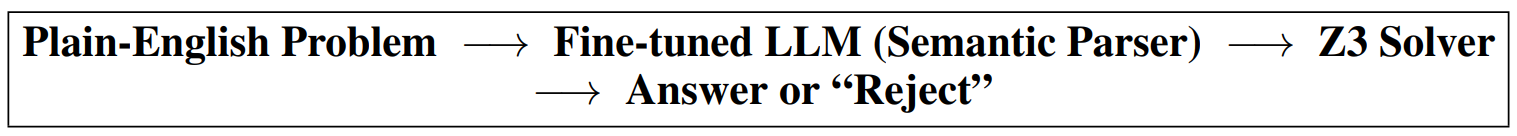
\includegraphics[width=\columnwidth]{pipeline.png}
  \caption{Overview of the proposed two-stage neuro-symbolic pipeline.}
  \label{fig:pipeline}
\end{figure}

\textbf{Stage 1: Language Model as a Translator.} The language model's role in this
system is not to solve the math problem directly. Instead, it will be trained to act as a
translator: given a problem written in plain English, it will produce a structured logical
description of that problem's variables and constraints in a format called
SMT-LIB~\cite{barrett2010}. SMT-LIB is a standardized text format used to describe
logical constraints, similar to how a programming language describes instructions for a
computer.

Standard language models are trained by repeatedly predicting the next word in a piece of
text~\cite{vaswani2017}. This system will use the same underlying training process, but
the target output will be changed from natural language to SMT-LIB code. This process is
called Supervised Fine-Tuning (SFT): the model is shown many (problem, SMT-LIB
description) pairs and learns to produce the correct logical description for each input.

The deep contextual representations (called embeddings) built up by the model's internal
attention layers~\cite{vaswani2017} are well-suited for capturing the relationships
between quantities and entities in a word problem. For example, understanding that
``John has three more apples than Mary'' implies the constraint $j = m + 3$.

\textbf{Stage 2: Constraint Solver as a Judge.} Once the language model produces an
SMT-LIB description, it will be passed to Z3~\cite{demoura2008}, a constraint-satisfaction
tool developed by Microsoft Research. Z3 checks whether the described constraints can all
be satisfied at the same time:

\begin{itemize}
  \item If Z3 finds a unique solution (\texttt{SAT}), that solution is returned as the
  final numeric answer.

  \item If Z3 determines the constraints are contradictory (\texttt{UNSAT}), the system
  will output \texttt{REJECT}, signaling a Contra-type ill-defined problem.

  \item If Z3 finds that infinitely many values satisfy the constraints, the system will
  also output \texttt{REJECT}, signaling a Missing-type ill-defined problem.
\end{itemize}

Because Z3 is a deterministic tool (it does not predict or guess, it proves), this
stage eliminates the possibility of the system hallucinating an answer at the reasoning
step.

\textbf{Handling Known Challenges.}

\begin{itemize}
  \item \textbf{Out-of-vocabulary (OOV) symbols:} Math problems frequently use unusual
  notation. The sub-word tokenization used by LLaMA-3 breaks unfamiliar symbols into
  smaller known pieces, reducing the impact of OOV terms. In addition, the normalization
  step described in Section~4 will standardize notation before tokenization.

  \item \textbf{Class imbalance:} The PMC dataset may contain unequal numbers of solvable
  vs.\ ill-defined problems. If this is the case, a weighted loss function will be used
  during training so that the model does not simply learn to predict the majority class.

  \item \textbf{Computational constraints:} LLaMA-3 is a large model. To make training
  feasible, Low-Rank Adaptation (LoRA)~\cite{hu2022} will be used, a technique that
  fine-tunes only a small fraction of the model's parameters while keeping the rest fixed.
  This reduces memory and time requirements significantly without sacrificing much
  performance.
\end{itemize}

%% ----------------------------------------------------------------
\section{Evaluation Plan}

The system will be evaluated along two dimensions: whether it correctly classifies
problems as solvable or not, and whether it produces the right numeric answer for solvable
ones.

\textbf{Primary metric: Classification Accuracy and F1 Score.} The main task is a
classification problem: given a math problem, the system must decide whether to solve it
or reject it. Accuracy will measure the overall percentage of correct decisions. Because
the classes may be imbalanced (more solvable problems than ill-defined ones), the F1 score
will also be reported. F1 is the harmonic mean of precision and recall, which penalizes a
system that achieves high accuracy by simply predicting the majority class most of the
time. A separate F1 score will be computed for each class (solvable, Missing-type,
Contra-type) to understand where the system struggles.

\textbf{Secondary metric: Answer Accuracy on Solvable Problems.} For problems the
system correctly identifies as solvable, the numeric answer produced by Z3 will be
compared against the ground-truth value. Since Z3 is a deterministic solver, any error
here will trace back to the language model producing an incorrect logical description.
This metric will help distinguish translation errors from classification errors.

\textbf{Baselines.} The results will be compared against two baselines to provide context:

\begin{itemize}
  \item \textbf{Vanilla LLaMA-3 (zero-shot):} The same base language model, prompted
  directly to answer the problem or say it cannot be solved, without any fine-tuning or
  external solver. This baseline shows the performance ceiling of a standard LLM on this
  task.

  \item \textbf{Chain-of-Thought LLaMA-3:} The same model prompted with step-by-step
  reasoning instructions~\cite{wei2022}. This baseline shows whether structured prompting
  alone is sufficient to handle ill-defined problems, without the overhead of a symbolic
  solver.
\end{itemize}

The proposed system is expected to outperform both baselines on ill-defined problem
detection, since neither baseline has a mechanism for formally verifying that a problem is
unsolvable. The comparison will show whether the added complexity of the symbolic solver
component is justified by a measurable improvement in F1.

%% ----------------------------------------------------------------
\bibliographystyle{ACM-Reference-Format}
\begin{thebibliography}{22}

\bibitem{brown2020}
T.~B. Brown, B.~Mann, N.~Ryder, M.~Subbiah, J.~Kaplan, P.~Dhariwal, et~al.
\newblock Language models are few-shot learners.
\newblock In \emph{Advances in Neural Information Processing Systems 33
  (NeurIPS 2020)}, 2020.

\bibitem{huang2025}
L.~Huang, W.~Yu, W.~Ma, W.~Zhong, Z.~Feng, H.~Wang, Q.~Chen, W.~Peng,
  X.~Feng, B.~Qin, and T.~Liu.
\newblock A survey on hallucination in large language models: Principles,
  taxonomy, challenges, and open questions.
\newblock \emph{ACM Transactions on Information Systems}, 43(2):1--55, 2025.

\bibitem{puchalska1987}
E.~Puchalska and Z.~Semadeni.
\newblock Children's reactions to verbal arithmetical problems with missing,
  surplus or contradictory data.
\newblock \emph{For the Learning of Mathematics}, 7(3):9--16, 1987.

\bibitem{wei2022}
J.~Wei, X.~Wang, D.~Schuurmans, M.~Bosma, B.~Ichter, F.~Xia, E.~Chi,
  Q.~Le, and D.~Zhou.
\newblock Chain-of-thought prompting elicits reasoning in large language
  models.
\newblock In \emph{Advances in Neural Information Processing Systems 35
  (NeurIPS 2022)}, pp. 24824--24837, 2022.

\bibitem{kojima2022}
T.~Kojima, S.~S. Gu, M.~Reid, Y.~Matsuo, and Y.~Iwasawa.
\newblock Large language models are zero-shot reasoners.
\newblock In \emph{Advances in Neural Information Processing Systems 35
  (NeurIPS 2022)}, pp. 22199--22213, 2022.

\bibitem{chen2023}
W.~Chen, X.~Ma, X.~Wang, and W.~W. Cohen.
\newblock Program of thoughts prompting: Disentangling computation from
  reasoning for numerical reasoning tasks.
\newblock \emph{Transactions on Machine Learning Research}, 2023.

\bibitem{imani2023}
S.~Imani, L.~Du, and H.~Shrivastava.
\newblock {MathPrompter}: Mathematical reasoning using large language models.
\newblock In \emph{Proceedings of the 61st Annual Meeting of the Association
  for Computational Linguistics (ACL 2023, Industry Track)}, pp. 37--42, 2023.

\bibitem{lightman2024}
H.~Lightman, V.~Kosaraju, Y.~Burda, H.~Edwards, B.~Baker, T.~Lee, J.~Leike,
  J.~Schulman, I.~Sutskever, and K.~Cobbe.
\newblock Let's verify step by step.
\newblock In \emph{Proceedings of the 12th International Conference on
  Learning Representations (ICLR 2024)}, 2024.

\bibitem{gao2023}
L.~Gao, A.~Madaan, S.~Zhou, U.~Alon, P.~Liu, Y.~Yang, J.~Callan, and
  G.~Neubig.
\newblock {PAL}: Program-aided language models.
\newblock In \emph{Proceedings of the 40th International Conference on Machine
  Learning (ICML)}, pp. 10764--10799. PMLR, 2023.

\bibitem{lu2023}
P.~Lu, B.~Peng, H.~Cheng, M.~Galley, K.-W. Chang, Y.~N. Wu, S.-C. Zhu,
  and J.~Gao.
\newblock Chameleon: Plug-and-play compositional reasoning with large language
  models.
\newblock In \emph{Advances in Neural Information Processing Systems 36
  (NeurIPS 2023)}, 2023.

\bibitem{yao2023}
S.~Yao, J.~Zhao, D.~Yu, N.~Du, I.~Shafran, K.~Narasimhan, and Y.~Cao.
\newblock {ReAct}: Synergizing reasoning and acting in language models.
\newblock In \emph{Proceedings of the 11th International Conference on
  Learning Representations (ICLR 2023)}, 2023.

\bibitem{schick2023}
T.~Schick, J.~Dwivedi-Yu, R.~Dess\`{i}, R.~Raileanu, M.~Lomeli, E.~Hambro,
  L.~Zettlemoyer, N.~Cancedda, and T.~Scialom.
\newblock Toolformer: Language models can teach themselves to use tools.
\newblock In \emph{Advances in Neural Information Processing Systems 36
  (NeurIPS 2023)}, pp. 68539--68551, 2023.

\bibitem{pan2023}
L.~Pan, A.~Albalak, X.~Wang, and W.~Y. Wang.
\newblock {Logic-LM}: Empowering large language models with symbolic solvers
  for faithful logical reasoning.
\newblock In \emph{Findings of the Association for Computational Linguistics:
  EMNLP 2023}, pp. 3806--3824, 2023.

\bibitem{ye2023}
X.~Ye, Q.~Chen, I.~Dillig, and G.~Durrett.
\newblock {SatLM}: Satisfiability-aided language models using declarative
  prompting.
\newblock In \emph{Advances in Neural Information Processing Systems 36
  (NeurIPS 2023)}, 2023.

\bibitem{demoura2008}
L.~de~Moura and N.~Bj{\o}rner.
\newblock {Z3}: An efficient {SMT} solver.
\newblock In \emph{Proceedings of the 14th International Conference on Tools
  and Algorithms for the Construction and Analysis of Systems (TACAS)},
  pp. 337--340, 2008.

\bibitem{heyueya2023}
J.~He-Yueya, G.~Poesia, R.~E. Wang, and N.~D. Goodman.
\newblock Solving math word problems by combining language models with symbolic
  solvers.
\newblock \emph{arXiv preprint arXiv:2304.09102}, 2023.

\bibitem{zhou2024}
S.-Y. Tian, Z.~Zhou, K.-Y. Yu, M.~Yang, L.-H. Jia, L.-Z. Guo, and Y.-F. Li.
\newblock {VCSearch}: Bridging the gap between well-defined and ill-defined
  problems in mathematical reasoning.
\newblock \emph{arXiv preprint arXiv:2406.05055}, 2024.

\bibitem{cobbe2021}
K.~Cobbe, V.~Kosaraju, M.~Bavarian, M.~Chen, H.~Jun, M.~Kaiser,
  M.~Plappert, J.~Tworek, J.~Hilton, R.~Nakano, C.~Hesse, and J.~Schulman.
\newblock Training verifiers to solve math word problems.
\newblock \emph{arXiv preprint arXiv:2110.14168}, 2021.

\bibitem{dubey2024}
A.~Dubey, A.~Jauhri, A.~Pandey, A.~Kadian, A.~Al-Dahle, A.~Letman, et~al.
\newblock The Llama 3 herd of models.
\newblock \emph{arXiv preprint arXiv:2407.21783}, 2024.

\bibitem{barrett2010}
C.~Barrett, A.~Stump, C.~Tinelli, et~al.
\newblock The {SMT-LIB} standard: Version 2.0.
\newblock In \emph{Proceedings of the 8th International Workshop on
  Satisfiability Modulo Theories (SMT)}, 2010.

\bibitem{vaswani2017}
A.~Vaswani, N.~Shazeer, N.~Parmar, J.~Uszkoreit, L.~Jones, A.~N. Gomez,
  {\L}.~Kaiser, and I.~Polosukhin.
\newblock Attention is all you need.
\newblock In \emph{Advances in Neural Information Processing Systems 30
  (NeurIPS 2017)}, 2017.

\bibitem{hu2022}
E.~J. Hu, Y.~Shen, P.~Wallis, Z.~Allen-Zhu, Y.~Li, S.~Wang, L.~Wang, and
  W.~Chen.
\newblock {LoRA}: Low-rank adaptation of large language models.
\newblock In \emph{Proceedings of the 10th International Conference on
  Learning Representations (ICLR 2022)}, 2022.

\end{thebibliography}

\end{document}